\documentclass{article}
\usepackage[utf8]{inputenc}% encodage du fichier source
\usepackage[francais]{babel}% rajouter éventuellement english, greek, etc.
\usepackage{listings}
\usepackage{hyperref}
\usepackage[margin=2.5cm]{geometry}
\usepackage{graphicx}
\hypersetup{urlcolor=,linkcolor=} % Does not apply color to href's
\lstset{
	tabsize=4,
	language=Java,
        basicstyle=\scriptsize,
        columns=fixed,
        extendedchars=true,
        breaklines=true,
		frame=single,
        showtabs=false,
        showspaces=false,
        showstringspaces=false,
        identifierstyle=\ttfamily,
        keywordstyle=\color[rgb]{0,0,1},
        commentstyle=\color[rgb]{0.133,0.545,0.133},
        stringstyle=\color[rgb]{0.627,0.126,0.941},
        numbers=left, 
        numberstyle=\tiny,
        xleftmargin=\parindent
}


\title{Android - TP2}
\date{Source, pdf et corrigé de ce TP
:\\ \href{http://tiny.cc/techmob}{http://tiny.cc/techmob}}

\begin{document}
\maketitle
L'objectif de ce TP est de réaliser une todo list (liste de choses à faire).\\
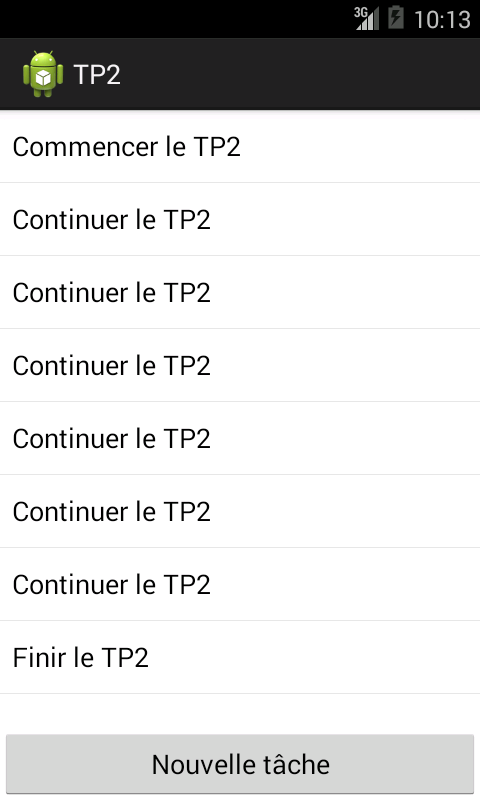
\includegraphics[width=100pt]{img/tp2screen1.png}
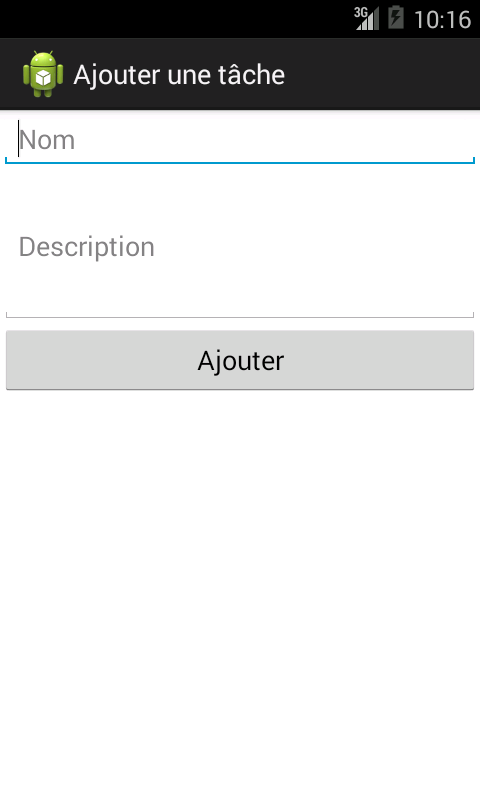
\includegraphics[width=100pt]{img/tp2screen2.png}
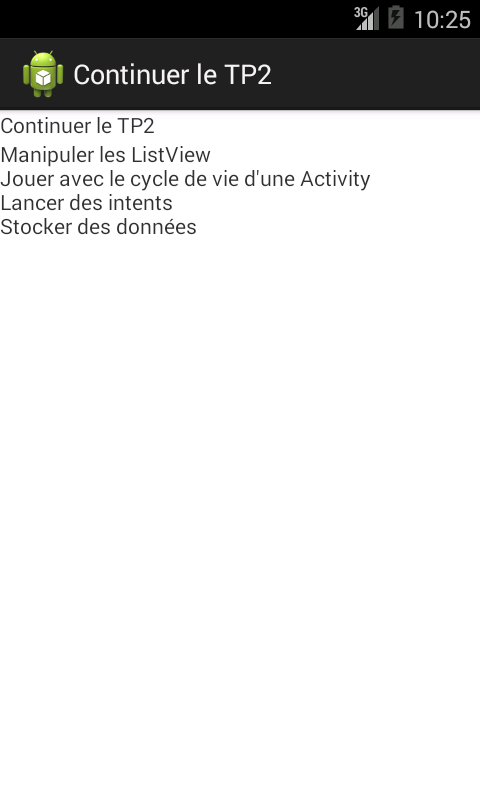
\includegraphics[width=100pt]{img/tp2screen3.png}\\
Ce TP fera appel aux notions suivantes :
\begin{itemize}
  \item ListView
  \item Listeners
  \item Cycle de vie de l'activity
  \item Intents
  \item Stockage de données
\end{itemize}
Il est fortement conseillé d'avoir le cours à portée de main et à ne pas hésiter
à se référer à la documentation officielle
\href{http://d.android.com}{http://d.android.com} ainsi que la multitude de tutoriaux disponibles.\\

\section{L'écran principal : affichage des tâches}
\begin{itemize}
  \item Créer un nouveau projet android avec une Activity simple (EmptyActivity)
  \item Modifier le layout de cette activity pour y placer une ListView qui
  prendra toute la largeur et toute la hauteur
\end{itemize}
\begin{enumerate}
 \setcounter{enumi}{0}
 \item Quel composant est chargé de faire le lien entre les données et la
 ListView ? (on l'implémentera plus tard)
 \end{enumerate}
 On souhaite ajouter un bouton ``ajouter une tâche'' en dessous de la ListView.
 \begin{enumerate}
 \setcounter{enumi}{1}
\item Pourquoi un LinearLayout ``naïf'' ne convient t'il pas ?
\item Pourquoi un RelativeLayout ne convient t'il pas totalement ?
\end{enumerate}
\begin{itemize}
  \item En utilisant la propriété layout\_weight de LinearLayout, placer le
  bouton en bas de l'écran.
  \item Ecouter les clicks sur le bouton et afficher un Toast à chaque click
\end{itemize}
\section{Un écran secondaire : ajout d'une tâche}
\begin{itemize}
  \item Créer une deuxième activity (rappel : ne pas oublier de l'ajouter au manifest !)
  \item Ajouter deux champs de texte modifiables (nom et commentaires) ainsi
  qu'un bouton ``ajouter'' à cette activity (libre à vous de définir le layout)
\end{itemize}
\section{Enchainement des écrans}
\subsection{Dans un sens \ldots}
\begin{enumerate}
 \setcounter{enumi}{4}
\item On veut lancer l'activity d'ajout d'une tâche lors d'un click sur le
bouton ``ajouter une tache'' de l'activity principale.
Quel concept android va-t-on utiliser ? (indice : il peut être soit implicite
soit explicite)
\item Dans ce cas, est-il implicite ou explicite ?
\item Pensez vous qu'il faille passer des données lors de l'appel à l'activity ``ajouter une tâche'' ? Si oui, lesquelles ?
\end{enumerate}
\begin{itemize}
  \item Lancer l'activity d'ajout de tâche lors d'un click sur le bouton.
\end{itemize}
\subsection{\ldots et dans l'autre}

Lors d'un click sur le bouton ``ajouter'' de l'activity d'ajout, on souhaite retourner à l'écran principal.
 \begin{enumerate}
 \setcounter{enumi}{7}
\item Est-il judicieux de lancer un intent vers l'activity principale ? 
\end{enumerate}
 En réalité, android construit une pile des activités lancées (stack). \href{http://developer.android.com/guide/components/tasks-and-back-stack.html}{Documentation officielle sur le stack} 
  \begin{itemize}
  \item En faire l'éxpérience en allant sur l'activity d'ajout puis en appuyant
  sur le bouton retour de l'appareil.
  \item Utiliser la méthode
  \href{http://developer.android.com/reference/android/app/Activity.html#finish()}{finish()} de Activity pour fermer l'activity et ainsi revenir à l'écran principal lors d'un click sur le bouton ajouter.
 \end{itemize}
 
 \section{Place aux données !}
 \begin{itemize}
  \item Créer une classe métier déstinée à contenir les données : Element.
  Chaque élément de la todo list contiendra au moins un nom et une description.
 \end{itemize}
 \subsection{Afficher les données dans la ListView}
    On ne souhaite afficher dans la liste que le nom des éléments.
      \begin{enumerate}
 \setcounter{enumi}{8}
\item Au vu de la simplicité des données à afficher pour chaque élément (un seul
champ de texte), quel type d'adapter vous parait le plus intéressant ? (Rappel :
on a le choix entre ArrayAdapter, CursorAdapter et faire sa propre implémentation à partir de BaseAdapter)
\end{enumerate}
 \begin{itemize}
  \item Dans onCreate : Créer une instance de l'adapter correspondant en
  utilisant comme layout pour chaque view le layout ``android.R.layout.simple\_list\_item\_1''
  \item Ouvrir le fichier XML de ce layout à l'aide de CTRL+click et constater
  sa simplicité
  \item Initialiser cet adapter avec une liste de Element générés à la volée
  \item Affecter cet adapter à la ListView
 \end{itemize}
  \subsection{Stocker les données}
  \begin{enumerate}
 \setcounter{enumi}{9}
\item Quelle solution de stockage des données vous parait la plus adaptée ?
(Rappel : on a le choix entre Preferences, fichier plat, base de données SQLite et stockage distant)
\end{enumerate}
 \begin{itemize}
  \item Pour des raisons de simplicité, on va opter dans la suite pour un stockage en fichier plat (libre à vous de le remplacer par une base SQLite)
  \item Créer une nouvelle classe ElementDAO qui se chargera des sauvegardes /
  chargements de données.
  \item Y créer une méthode qui écrit une liste d'éléments Element dans un
  fichier en utilisant un format de stockage primitif par exemple
  nom\#description et un Element par ligne.
  \\Note : Ce format est un très mauvais choix en pratique car peu robuste et
  peu extensible mais suffira largement ici.
  \item Créer une méthode qui instancie une liste d'Element à partir des valeurs
  lues dans le fichier.
  \item Dans la méthode onCreate(), remplir la ListView à partir des données contenues dans le fichier.
 \end{itemize}
 \subsection{Remplir les données}
 \begin{itemize}
  \item Lors d'un click sur le bouton ``ajouter'' de l'activity d'ajout, créer
  une instance d'Element et la rajouter au fichier. (pour simplifier, réécrire
  la totalité du fichier à chaque fois)
 \end{itemize}
  \begin{enumerate}
 \setcounter{enumi}{10}
\item Pourquoi la ListView n'est elle pas mise à jour lors du retour sur l'activity principale ?
\end{enumerate}
 \begin{itemize}
  \item Utiliser le cycle de vie des activities pour recharger les données de la ListView lors du retour sur l'activity principale. (implémenter la bonne méthode onXXXXX)
 \end{itemize}
 \section{Voir le détail d'un élément}
 \begin{itemize}
  \item Créer une activity de visualisation d'item avec les champs utiles (nom, description \ldots)
  \item Récupérer les clicks sur les éléments de la ListView (Attention à bien utiliser onItemClickListener et non onClickListener).
  \item Lancer l'activity de visualisation lors d'un click sur un item de la liste
  \item Transmettre à l'activity le nom de l'item choisi
  \item Récupérer les données dans l'activity de visualisation et afficher les
  données de l'élément
 \end{itemize}
 \section{Pour aller plus loin}
	Wow, déjà tout fait ? Voici quelques pistes d'améliorations :
  \begin{itemize}
  \item Le stockage en fichier plat n'est pas très judicieux. Mettre en place une base de données SQLite à la place.
  \item Les données associées aux items sont pour l'instant minimales, pourquoi ne pas ajouter un identifiant, une date d'ajout, un statut (en cours, fait \ldots), une priorité, une catégorie \ldots ?
  \item L'affichage des éléments dans la liste est basique mais on peut difficilement faire mieux avec ArrayAdapter. Créer un adapter maison en héritant de BaseAdapter
  \item Partager les items par mail, sms, twitter \ldots en ajoutant un intent implicite dans l'activity de visualisation ou de modification.
 \end{itemize}
\end{document}


